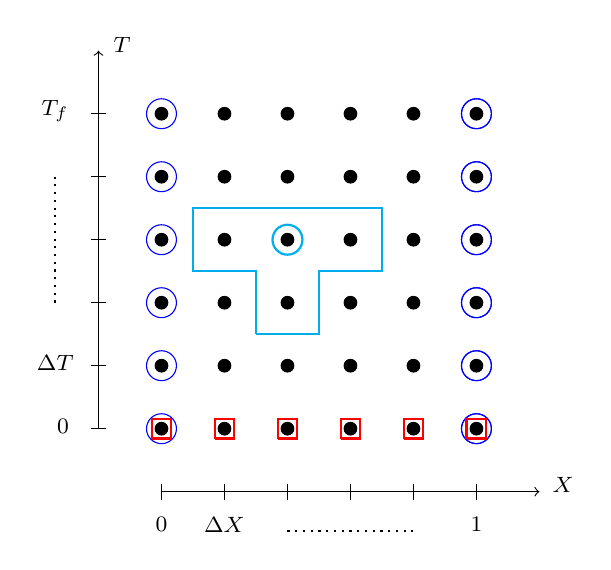
\begin{tikzpicture}
  \foreach \x in {0,...,5}{
      \draw (-0.9,\x*0.8)--(-0.7,\x*0.8);
      \draw (\x*0.8,-0.9)--(\x*0.8,-0.7);
      \foreach \y in {0,...,5}
      \draw[black,fill=black] (0.8*\y,0.8*\x) circle (0.08cm);}
  \draw [->](-0.8,0)--(-0.8,0.8*5+0.8);
  \node[anchor=north,font=\footnotesize] at (-0.5,0.8*5+1.1) {$T$};
  \draw [->](0,-0.8)--(0.8*5+0.8,-0.8);
  \node[anchor=north,font=\footnotesize] at (0.8*5+1.1,-0.5) {$X$};
  \node[anchor=north,font=\footnotesize] at (0,-1) {$0$};
  \node[anchor=north,font=\footnotesize] at (0.8,-1) {$\Delta X$};
  \draw[thick, dotted] (1.6,-1.3) -- (3.2,-1.3);
  \node[anchor=north,font=\footnotesize] at (-1.35,4.3) {$T_f$};
  \node[anchor=north,font=\footnotesize] at (-1.25,0.25) {$0$};
  \node[anchor=north,font=\footnotesize] at (-1.35,1.05) {$\Delta T$};
  \draw[thick, dotted] (-1.35,1.6) -- (-1.35,3.2);
  \node[anchor=north,font=\footnotesize] at (4,-1) {$1$};
  \pgfmathsetmacro{\R}{0.19}
  \pgfmathsetmacro{\D}{0.25}
  \foreach \x in {0,...,5}{
      \draw[blue] (0,0.8*\x) circle (\R cm);
      \draw[blue] (4,0.8*\x) circle (\R cm);
      \draw[blue] (4,0.8*\x) circle (\R cm);
      \draw[red, thick] (0.8*\x-\D/2,0-\D/2) -- (0.8*\x-\D/2,0+\D/2) -- (0.8*\x+\D/2,0+\D/2) -- (0.8*\x+\D/2,0-\D/2)--(0.8*\x-\D/2,0-\D/2);}
  \draw[cyan, thick] (1.6,2.4) circle (\R cm);
  \draw[cyan, thick] (1.2,1.2) -- (2,1.2) -- (2,2) -- (2.8,2) -- (2.8,2.8) -- (0.4,2.8) -- (0.4,2) -- (1.2,2) -- (1.2,1.2);
\end{tikzpicture}
